The FMM as originally presented has since been extended into a broad class of algorithms with differing implications for practical implementations. We consider the problem in its most generic form by returning to the matrix vector product (\ref{eq:ch_1:n_body}). We consider a non-oscillatory problem with a Laplace kernel from electrostatics to introduce the ideas behind the FMM as in the original presentation \cite{greengard1987fast}. Given an $N$-body evaluation of electrostatic potentials, we let $\{ x_i\}_{i=1}^N \in \mathbb{R}^d$ denote the set of locations of charges of strength $q_i$, where $d=2$ or $d=3$. Our task is then to evaluate potentials, $\phi_j$ for $i=1,2,...,N$. Without loss of generality we take the value of $K(x,x)=0$. Denoting a square/cube domain containing all points with $\Omega$, we seek to evaluate a matrix vector product of the form,

\begin{flalign}
    \label{eq:ch_2:potential_matvec}
    \mathsf{\phi} = \mathsf{K} \mathsf{q}
\end{flalign}

where $\mathsf{\phi} \in \mathbb{C}^N$, $\mathsf{q} \in \mathbb{C}^N$ and $\mathsf{K} \in \mathbb{C}^{N \times N}$. The idea is to compress the kernel interactions defined by $K(x,y)$ when $x$ and $y$ are distant. Consider the situation in figure (\ref{fig:ch_2:single_level_r2}) where we choose $\mathbb{R}^2$ for simplicity. Here we seek to evaluate the potential induced by the source particles, $\{y_j\}_{j=1}^M$, in $\Omega_s$ at the target particles, $\{x_i\}_{i=1}^L$ in $\Omega_t$.

\begin{flalign}
    \label{eq:ch_2:two_box_calc}
    \phi_i = \sum_{j=1}^L K(x_i, y_j) q_j, \> \> i=1,2...M
\end{flalign}

As the sources and targets are physically distant, we can apply a low-rank approximation for the kernel as a sum of tensor products,

\begin{flalign}
    K(x,y) \approx \sum_{p=0}^{P-1}B_p(x)C_p(y), \> \> \text{when } x \in \Omega_t, y \in \Omega_s 
    \label{eq:ch_2:low_rank_decomposition_of_kernel}
\end{flalign}

where $P$ is called the `expansion order', or `interaction rank'. We introduce the index sets $I_s$ and $I_t$ which list the points inside $\Omega_s$ and $\Omega_t$ respectively, and consider a generic approximation by tensor products where,

\begin{flalign}
    \hat{q}_p = \sum_{j \in I_s} C_p(x_j)q_j, \> \> p = 0,1,2,...,P-1
\end{flalign}

this is a good approximation, as low-rank approximation of $K$ converges rapidly in the far-field. Using this, we evaluate the approximation of the potential at the targets as,

\begin{flalign}
    \label{eq:ch_2:low_rank_appx}
    \phi_i \approx \sum_{p=1}^{P-1} B_p(x_i)\hat{q}_p
\end{flalign}

In doing so we see that we accelerate (\ref{eq:ch_2:two_box_calc}) from $O(ML)$ to $O(P(M+L))$. As long as we choose $P \ll M$ and $P \ll L$, we will recover an accelerated matrix vector product. The power of the FMM, and similar fast algorithms, is that we can recover the potential in $\Omega_t$ with high accuracy even when $P$ is small.

We deliberately haven't stated how we calculate $B_p$ or $C_p$. In Greengard and Rokhlin's FMM these took the form of analytical multipole and local expansions of the kernel function \cite{greengard1987fast}. To demonstrate this we derive an expansion in the $\mathbb{R}^2$ case, taking $c_s$ and $c_t$ as the centres of $\Omega_s$ and $\Omega_t$ respectively,

\begin{flalign}
    \label{eq:ch_2:analytical_multipole_expansion}
    K(x,y) = \log(x-y) &= \log((x-c_s) - (y-c_s)) \\ \nonumber &= \log(x-c_s) + \log(1-\frac{y-c_s}{x-c_s}) \\
    \nonumber &= \log(x-c_s) - \sum_{p=1}^\infty \frac{1}{p}\frac{(y-c_s)^p}{(x-c_s)^p}
\end{flalign}

where the series converges for $|y-c_s| < |c-c_s|$. We note (\ref{eq:ch_2:analytical_multipole_expansion}) is exactly of the form required with $C_p(y) = -\frac{1}{p}(y-c_s)^p$ and $B_p(x) = (x-c_s)^{-p}$. We define a `multipole expansion' of the charges in $\Omega_s$ as a vector $\mathsf{\hat{q}^s} = \{ \hat{q}_p^s \}_{p=0}^{P-1}$,

\begin{flalign}
    \begin{dcases}
        \hat{q}_0^s = \sum_{j \in I_s} q_j \\ 
        \hat{q}_p^s = \sum_{j \in I_s} - \frac{1}{p}(x_j - c_s)^p q_j, \> \> p = 1,2,3...,P-1
    \end{dcases}
\end{flalign}

The multipole expansion is a representation of the charges in $\Omega_s$ and can be truncated to any required precision. We can use the multipole expansion in place of a direct calculation with the particles in $\Omega_s$. As the potential in $\Omega_t$ can be written as,

\begin{flalign}
    \phi(x) = \sum_{j \in I_s} K(x, y)q_j = \log(x-c_s)\hat{q}_0^s + \sum_{p=1}^\infty \frac{1}{(x-c_s)^p}\hat{q}_p^s
    \label{eq:ch_2:multipole_expansions}
\end{flalign}

Greengard and Rokhlin also define a local expansion centered on $\Omega_t$, that represents the potential due to the sources in $\Omega_s$.

\begin{flalign}
    \phi(x) = \sum_{l=1}^\infty (x-c_t)^l \hat{\phi}^t_l
\end{flalign}

with a simple computation to derive the local expansion coefficients $\{\hat{\phi}^t_p\}_{p=0}^\infty$ from $\{ \hat{q}_p^s \}_{p=0}^{P-1}$ (see app. \ref{app:a_1_fmm_algorithm}).

For our purposes it's useful to write the multipole expansion in linear algebraic terms as a linear map between vectors,

\begin{flalign}
    \mathsf{\hat{q}}^s = \mathsf{T}^{P2M}_s\mathsf{q}(I_s)    
\end{flalign}

where $\mathsf{T}_s^{P2M}$ is a $P \times N_s$ matrix, analogously for the local expansion coefficients we can write,

\begin{flalign}
    \mathsf{\hat{\phi}}^t = \mathsf{T}_{t,s}^{M2L}\mathsf{\hat{q}}^s
\end{flalign}

where $\mathsf{T}_{t,s}^{M2L}$ is a $P \times P$ matrix, and the calculation of the final potentials as,

\begin{flalign}
    \mathsf{\phi}^t = \mathsf{T}_t^{L2P}\mathsf{\hat{\phi}}^t
\end{flalign}

where $\mathsf{T}_t^{L2P}$ is a $N_t \times P$ matrix. Here we denote each \textit{translation} operator, $\mathsf{T}^{X2Y}$, with a label read as `$X$ to $Y$' where $L$ stands for local, $M$ for multipole and $P$ for particle. Written in this form, we observe that one could use a different method to approximate the translation operators than explicit kernel expansions to recover our approach's algorithmic complexity, and this is indeed the main difference between different implementations of the FMM.

We have described how to obtain linear complexity when considering two isolated nodes, however in order to recover this for interactions between \textit{all particles} with we rely on a hierarchical partitioning of $\Omega$ using a data structure from computer science called a \textit{quadtree} in $\mathbb{R}^2$ or an \textit{octree} in $\textit{R}^3$. The defining feature of these data structures is a recursive partition of a bounding box drawn over the region of interest (see fig. \ref{fig:ch_2:octree_example}). This ‘root node’ is subdivided into four equal parts in $\mathbb{R}^2$ and eight equal parts in $\mathbb{R}^3$. These ‘child nodes’ turn are recursively subdivided until a user defined threshold is reached based on the maximum number of points per leaf node. These trees can be `adaptive' by allowing for non-uniform leaf node sizes, and `balanced' to enforce a maximum size constraint between adjacent leaf nodes \cite{sundar2008bottom}.

\begin{figure}
    \centering
    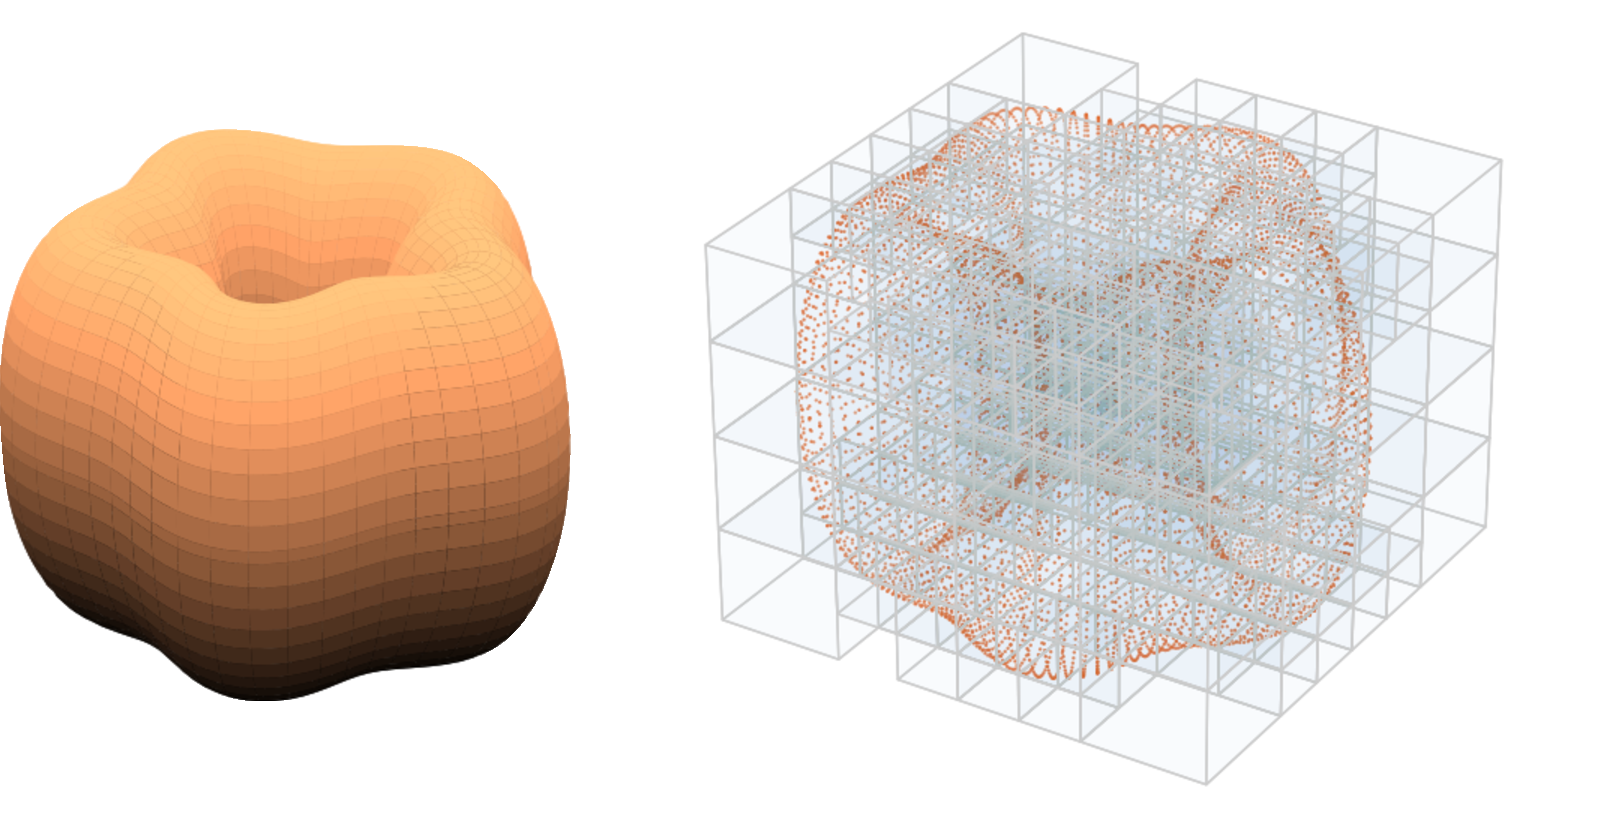
\includegraphics[width=0.7\textwidth]{ch_2/octree_example.pdf}
    \caption{An adaptive octree for random point data placed on the surface of a `wiggly torus' test geometry. The user defines the level of recursion via a threshold for the maximum number of particles in a given node.}
    \label{fig:ch_2:octree_example}
\end{figure}

In addition to the $\mathsf{T}^{P2M}$, $\mathsf{T}^{M2L}$ and $\mathsf{T}^{L2P}$ the FMM also require operators that can translate the expansion centre of a multipole or local expansion, $\mathsf{T}^{L2L}$, $\mathsf{T}^{M2M}$, an operator that can form a local expansion from a set of points $\mathsf{T}^{P2L}$, and apply a multipole approximation to a set of points, $\mathsf{T}^{M2P}$, finally we need define a $P2P$ operator, which is short hand for direct kernel evaluations. Algorithm (\ref{alg:ch_2:fmm}) provides a brief sketch of the full FMM algorithm which combines these operators.

\begin{algorithm}
\caption{\textbf{Adaptive Fast Multipole Method}: FMM literature distinguishes between types of relationships  between neighbouring nodes with the concept of \textit{interaction lists}. There are four such lists for a given node $B$, called $V$, $U$, $W$ and $X$. For a leaf node $B$, the $U$ list contains $B$ itself and leaf nodes adjacent to $B$. and the $W$ list consists of the descendants of $B$'s neighbours whose parents are adjacent to $B$. For non-leaf nodes, the $V$ list is the set of children of the neighbours of the parent of $B$ which are not adjacent to $B$, and the $X$ list consists of all nodes $A$ such that $B$ is in their $W$ lists. The non-adaptive algorithm is similar, however the $W$ and $X$ lists are empty.}
\label{alg:ch_2:fmm}
\begin{algorithmic}

    \STATE $N$ is the total number of points
    \STATE $s$ is the maximum number of points in a leaf node.

    \STATE
    \STATE \textbf{Step 1: Tree construction}
    
    \FOR{each node $B$ in \textit{preorder} traversal of tree, i.e. the nodes are traversed bottom-up, level-by-level, beginning with the finest nodes.}
        \STATE subdivide $B$ if it contains more than $s$ points.
    \ENDFOR
    \FOR{each node $B$ in \textit{preorder} traversal of tree}
        \STATE construct \textit{interaction lists}, $U$, $V$, $X$, $W$
    \ENDFOR
    
    \STATE 
    \STATE \textbf{Step 2: Upward Pass}
    \FOR{each leaf node $B$ in \textit{postorder} traversal of the tree, i.e. the nodes are traversed top-down, level-by-level, beginning with the coarsest nodes.}
    \STATE \textbf{P2M}: compute multipole expansion for the particles they contain.
    \ENDFOR
    \FOR{each non leaf node $B$ in \textit{postorder} traversal of the tree}
    \STATE \textbf{M2M}: form a multipole expansion by translating the expansion centre of its children to its centre and summing their multipole expansion coefficients.
    \ENDFOR

    \STATE
    \STATE \textbf{Step 3: Downward Pass}
    \FOR{each non-root node $B$ in \textit{preorder} traversal of the tree}
    \STATE \textbf{M2L}: translate multipole expansions of nodes in $B$'s $V$ list to a local expansion at $B$.
    \STATE \textbf{P2L}: translate the charges of particles in $B$'s $X$ to the local expansion at $B$.
    \STATE \textbf{L2L}: translate $B$'s local expansion to its children by translating its expansion centre to the centre of its children, and assigning the same coefficients.
    \ENDFOR 

    \FOR{each leaf node $B$ in \textit{preorder} traversal of the tree}
    \STATE \textbf{P2P}: directly compute the local interactions using the kernel between the particles in $B$ and its $U$ list.
    \STATE \textbf{L2P}: translate local expansions for nodes in $B$'s $W$ list to the particles in $B$.
    \STATE \textbf{M2P}: translate the multipole expansions for nodes in $B$'s $W$ list to the particles in $B$.
    \ENDFOR
\end{algorithmic}
\end{algorithm}

\begin{figure}
    \centering
    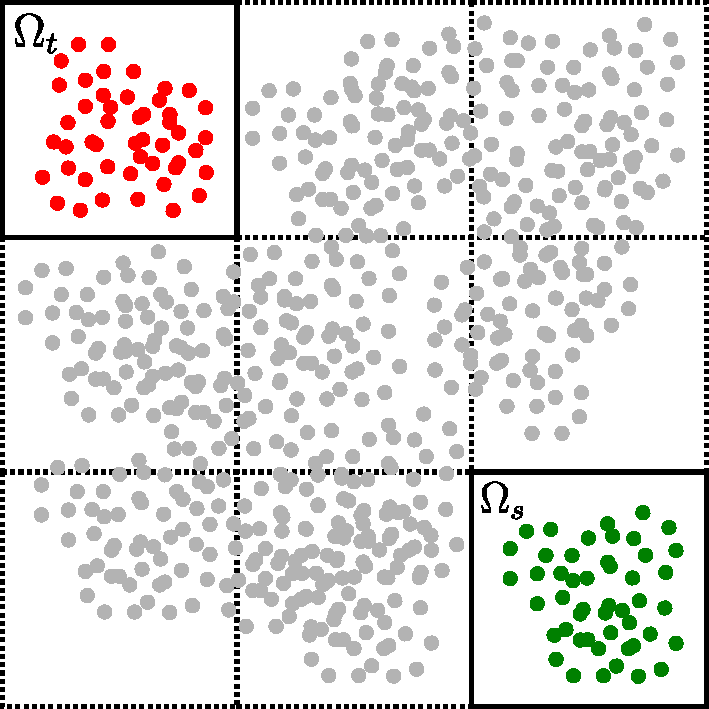
\includegraphics[width=0.5\textwidth]{ch_2/single_level_r2.pdf}
    \caption{Two well separated clusters $\Omega_t$ and $\Omega_s$ where we can apply a low-rank approximation.}
    \label{fig:ch_2:single_level_r2}
\end{figure}

In its original analytical form the applicability of the FMM is limited by the requirement for an explicit multipole and local expansions, as well as a restriction to matrix vector products. Concurrently to the development of the FMM, algebraic analogues were developed. These methods are mathematically equivalent, similarly based on a hierarchical partition of the point data using a recursive tree, and an admissibility condition. The underlying difference being in how they represent field expansions, which are no longer required to be multipole expansions, as well as the translation operators and their representation of the field translations in as an explicit matrix acting on the point charges and their multipole and local expansion coefficients. Once this representation is computed it can be used again allowing for simple extensions to matrix-matrix products. The explicit expression as a matrix also allows for algorithms that can operate on this data structure to approximate the matrix inverse. Examples of algebraic matrix representations include the $\mathcal{H}$ matrix \cite{hackbusch1999sparse}, $\mathcal{H}^2$ matrix \cite{borm2003short}, hierarchically semi-separable (HSS) \cite{chandrasekaran2007fast}, and hierarchically off-diagonal low-rank (HODLR) \cite{ambikasaran2013mathcal} matrices. 

Consider an index set $I$, corresponding to the indices of all points $\{ x_i \}_{i=1}^N$ in a given discretisation. The general approach of these methods is to partition $I$ in such a way that we can exploit the low-rank interactions between distantly separated clusters of particles. We identify this `cluster tree' approach as being analogous to the octree used in the analytical FMM. Initially, an binary `cluster tree' $\mathcal{T}_I$, with a set of nodes $T_I$, is formed such that

\begin{enumerate}
    \item $T_I \subseteq \mathcal{P}(I) \setminus \{ \emptyset \}$, meaning each node  of $\mathcal{T}_I$ is a subset of the index set $I$, here $\mathcal{P}(I)$ denotes the power set of $I$.
    \item $I$ is the root of $\mathcal{T}_I$
    \item The number of indices in a leaf node $\tau \in T_I$ is such that $|\tau| \leq C_{\text{leaf}}$ where $C_{\text{leaf}}$ is a small constant.
    \item Non leaf nodes $\tau$ have $n$ child nodes $\{ \tau \}_i^n$, and is formed of their disjoint union $\tau = \cupdot_{i=1}^n \tau_i$ 
\end{enumerate}

Using a cluster tree, one forms a `block tree', $\mathcal{T}_{I \times I}$. Each node, or `block', of a block tree, $N(\tau \times \sigma)$, corresponds to the clusters represented by indices $\tau \subseteq I$ and $\sigma \subseteq I$ respectively. The $\mathcal{H}$ and $\mathcal{H}^2$ representations are `strongly admissible', meaning that well separated blocks as in figure (\ref{fig:ch_1:low_rank}) can be compressed. In contrast, the HSS and HODLR approaches are `weakly admissible', and also consider adjacent clusters to be compressible. Admissibility is calculated by forming a bounding box around clusters, and checking their separation along each dimension \cite{borm2003introduction}. Furthermore, as in the FMM which creates parent multipole expansions for a given node from that of its children, and vice versa for local expansions, an analagous approach is taken by $\mathcal{H}^2$ and HSS matrices, referred to as `nested bases'. These different approaches are succinctly visualised in figure (\ref{fig:ch_2:ambikasaran_hierarchical}).  Expressed in this way the matrix implicit in the FMM (alg. (\ref{alg:ch_2:fmm})), can be seen to be a member of the $\mathcal{H}^2$ class of matrices. Therefore the algorithms developed for algebraic approaches for matrix vector products similarly recover optimal $O(N)$ scaling in the best case, with the additional benefit of easy extension to matrix matrix products, and matrix inversion in optimal complexity \cite{borm2003introduction}.

\begin{figure}
    \centering
    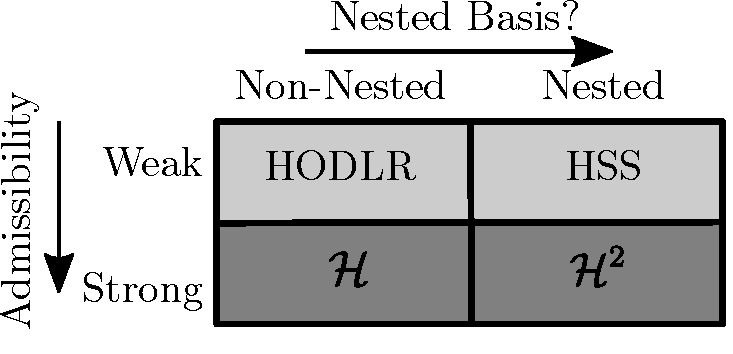
\includegraphics[width=0.5\textwidth]{ch_2/ambikasaran_hierarchical.pdf}
    \caption{Matrix containing common algebraic alternatives to the FMM, adapted from \cite{ambikasaran2013fast}.}
    \label{fig:ch_2:ambikasaran_hierarchical}
\end{figure}

From a computational perspective, the trade-off between these analytical and algebraic approaches for the FMM are best expressed in terms of the ratio of compute (flops) to memory (bytes), or `arithmetic intensity'. The analytical FMM has a high arithmetic intensity, due to its matrix free nature. However, using explicit $\mathcal{H}^2$ representations requires one to compute and store the full hierarchical matrix in memory, resulting in increased memory movement costs, both vertically on a single node, and horizontally in a distributed memory setting. 

Similar algebraic approaches, confusingly labelled `black box' FMMs combine the algorithmic structure of the analytical FMM with alternative field representations that aren't necessarily multipole expansions \cite{Ying:2004:JCP,fong2009black,martinsson2007accelerated}. The origin of the label `black box' is due to to the fact that the low rank representations they construct are done so independently of the kernel. We contrast two common black box methods in box (\ref{box:ch_2:kifmm_vs_bbfmm}), the underlying difference being in their representation of translation operators. Black box methods are preferable from a software standpoint for three reasons:

\begin{enumerate}
    \item Generic software interfaces can be built for a variety of kernels, unlike for analytical FMMs, as demonstrated by \cite{wang2021exafmm,kailasa2022pyexafmm}.
    \item They have reduced storage requirements in comparison to purely algebraic approaches.
    \item The majority of computations are simple matrix vector products that are readily expressed with BLAS L2 operations, and therefore maximise cache efficiency
\end{enumerate}

We emphasise that it is possible to extend the analytical FMM to more general kernels, such as the modified Laplacian \cite{greengard2002new}, Stokes \cite{fu2000fast} and Navier \cite{fu1998fast}, however software implementations are cumbersome, requiring the optimised calculation of special functions such as spherical harmonics, and are difficult to generalise for different problem settings. We have preferentially implemented the Kernel-Independent FMM of Ying et. al \cite{Ying:2004:JCP} in our previous software \cite{kailasa2022pyexafmm} as it has a particularly simple mathematical structure, and extends to a variety of kernels for elliptic partial differential equations of interest. Specifically, the Laplace, Stokes and Navier kernels alongside their modified variants \cite{Ying:2004:JCP}, as well as the Helmholtz kernel in the low-frequency setting \cite{wang2021exafmm}. 

\subsection*{Computational Considerations for the FMM}

In terms of algorithm optimisation significant efforts have gone towards optimising $T^{M2L}$ \cite{messner2012optimized,fong2009black,Ying:2004:JCP}, which is the most time consuming translation operator. It is computed for each non-leaf node between level one and the leaf level of a tree, it therefore grows as $O(N)$. In $\mathbb{R}^3$, the $V$ list for a node, containing its parent’s neighbors' children that are non-adjacent to the node, can be up to $|V| = 6^3 - 3^3=189$. However if a kernel exhibits translational invariance, such that

\begin{flalign*}
    K(x, y) = K(x-y)
\end{flalign*}

which is the case for the kernels mentioned above, we recognise that there are just $7^3-3^3=316$ unique $T^{M2L}$ operators per level. However, Messner et. al \cite{messner2012optimized} show that even these 316 operators are permutations of a subset of only 16 unique operators. Permutations corresponding to reflections across various planes (for example $x = 0$, $y = 0$, $z = 0$, etc). We can therefore write a block matrix of \textit{all} unique $T^{M2L}$ for a given level,

\begin{flalign}
    T^{M2L} = \left [ T^{M2L}_1 | T^{M2L}_2 | ... | T^{M2L}_{16} \right ]
    \label{eq:ch_2:m2l_stacked}
\end{flalign}

where $T^{M2L}_i$ corresponds to the $i^{\text{th}}$ \textit{transfer vector} describing a unique $T^{M2L}$. This block matrix is efficiently compressed using a truncated SVD, which is known to produce an optimal low rank approximation of a rank $N$ matrix, where the new rank, $r$, is chosen such that $r \ll N$. This is a common optimisation used in both black box \cite{Ying:2004:JCP,fong2009black} and analytical FMMs \cite{gimbutas2003generalized}. By precomputing and storing a compressed $T^{M2L}$ for each level, the $T^{M2L}$ operator for each node can be formed as a single BLAS level 2 operation at runtime by looking up the relevant compressed operators corresponding to its $V$ list. The $T^{M2M}$, $T^{L2L}$ can be similarly stored on a level by level basis, reducing the pre-computation time for operators to $O(d)$, where $d$ is the depth of an quad/octree. For homogenous kernels, for which, 

\begin{flalign*}
    K(\alpha x, \alpha y) = \alpha^m K(x, y)
\end{flalign*}

pre-computations can performed for a single level, and scaled to different levels, reducing pre-computation complexity to $O(1)$. Such optimisations further separate runtime performance between implementations of algebraic and black box methods, as the transfer operators $T^{M2L}$ correspond to duplicate blocks in an algebraic $\mathcal{H}^2$ which are redundantly computed and stored in implementations \cite{ghyselsstrumpack}.

\subsection*{Parallelising the KIFMM}

The computational complexities of KIFMM operators are defined by a user specified $n_{crit}$, which is the maximum allowed number of particles in a leaf node, $n_e$ and $n_c$ which are the numbers of quadrature points on the \textit{check} and \textit{equivalent} surfaces respectively (see sec. 3 \cite{Ying:2004:JCP}). The parameters $n_e$ and $n_c$ are quadratically related to the expansion order, i.e. $n_e = 6(p-1)^2 + 2$ \cite{Ying:2004:JCP}. Typical values for $n_{crit}$ used are $\sim 100$. Notice the depth of the octree is defined $n_{crit}$, and hence by the particle distribution.

The near field calculated directly using $P2P$, $T^{P2M}$, $T^{P2L}$, $T^{M2P}$, and $T^{L2P}$ operate independently over the leaf nodes. The $T^{M2L}$ and $T^{L2L}$ operate independently on all nodes at a given level, from level 2 to the leaf level, during the top-down traversal. The $T^{M2M}$ is applied to each node during the bottom-up traversal. All operators, except the $T^{M2L}$, $T^{M2M}$ and $T^{L2L}$, rely on the $P2P$. 

As explained in algorithm \ref{alg:ch_2:fmm}, the inputs to the M2L, M2P, P2L and near field operators are defined by `interaction lists' called the $V$, $W$, $X$ and $U$ lists respectively.  These interaction lists define the nodes a target node interacts with when an operator is applied to it. We can restrict the size of these interaction lists by demanding that neighboring nodes at the leaf level are at most twice as large as each other \cite{sundar2008bottom}. Using this `balance condition', the $V$, $X$, $W$ and $U$ lists in 3D contain at most 189, 19, 148 and 60 nodes, respectively.

The near field operator applies the $P2P$ between the charges contained in the target and the source particles of nodes in its $U$ list, in $O(60 \cdot n_{crit}^2)$. The $T^{M2P}$ applies the $P2P$ between multipole expansion coefficients of source nodes in the target's $W$ list and the charges it contains internally in $O(148 \cdot n_e \cdot n_{crit})$. Similarly, the $T^{L2P}$ applies the $P2P$ between a target's own local expansion coefficients and the charges it contains in $O(n_e \cdot n_{crit})$.

The $T^{P2L}$, $T^{P2M}$ and $T^{M2L}$ involve creating local and multipole expansions, and rely on a matrix vector product related to the number of source nodes being compressed, which for the $T^{P2L}$ and $T^{M2L}$ are defined by the size of the target node's interaction lists. These matrix vector products have complexities of the form $O(k \cdot n_e^2)$ where $k = |X| = 19$ for the $T^{P2L}$, $k = |V| = 189$ for the $T^{M2L}$, and $k = 1$ for the P2M. Additionally, the $T^{P2L}$ and $T^{P2M}$ have to calculate `check potentials' (see sec. box (\ref{box:ch_2:kifmm_vs_bbfmm})) which require $O(19 \cdot n_{crit} \cdot n_c)$ and $O(n_{crit} \cdot n_c)$ calculations respectively. The $T^{M2M}$ and $T^{L2L}$ operators both involve translating expansions between nodes their eight children, and rely on a matrix vector product of $O(n_e^2)$.

The structure of the FMM's operators expose natural parallelism. The $P2P$ is embarrassingly parallel over each target. As are the $T^{M2L}$, $T^{M2P}$, $T^{P2L}$ and near field operators over their interaction lists. The near field, $T^{L2P}$, $T^{M2P}$, $T^{P2L}$ and $T^{P2M}$ operators are also embarrassingly parallel over the leaf nodes, as are the $T^{M2L}$, $T^{M2M}$ and $T^{L2L}$ over the nodes at a given level.

\subsection*{Conclusion}

A significant challenge in practical FMM implementations is handling the global data dependency encapsulated in (\ref{eq:ch_2:two_box_calc}). Historical single-core architectures have always suffered from the Von Neumann bottleneck, whereby data is loaded from main memory slower than the processor is able to absorb it. However, with the breakdown of Dennard scaling\footnote{Dennard Scaling is the insight that the power density of transistors appeared to remain constant as they grew smaller.} from around 2006 and the subsequent multicore revolution the disparity between data movement costs and computation have been even further exacerbated. On modern hardware accelerators are able to achieve $O(1e12)$ flop rates in double precision, but are bandwidth limited to $O(1e11)$ bytes/second, meaning that an order of magnitude more operations have to performed for every byte retrieved from memory, to remain efficient. Dongarra et. al \cite{dongarra2017extreme}, go as far as to suggest that the dominant role of communication costs on emerging hardware, especially in the context of exascale architectures, mean that complexity analysis of distributed algorithms based on flop counts are redundant entirely. Indeed, in a distributed memory setting global reductions are often the largest performance limiting factor \cite{dongarra2017extreme}. The data dependency of the FMM is expressed in the quad/octree, with significant global reductions required for translation operators. It is therefore critical to implement highly optimised algorithms for tree construction in a distributed setting, however we defer a discussion on this until chapter \ref{chpt:6:rusty_tree}.

We conclude by mentioning that the FMM and its variants are not the only technique available to accelerate (\ref{eq:ch_1:n_body}), for problems in which only uniform resolution is required the FFT, which has corresponding distributed memory implementations \cite{gholami2015accfft}. However, we are commonly interested in multiscale problems in which neighbouring nodes can be of differing sizes. In this setting, multigrid methods have shown slower convergence in comparison to the FMM \cite{yokota2015fast,gholami2016fft}. Furthermore, a multigrid approach does not allow for a re-use of FMM data structures for other fast algorithms we are interested in implementing, and aim to present as a unified framework with maximum code re-use. We observe that the choice between analytical, black box and algebraic FMM variants may have a significant impact on the ultimate implementation, and performance, this is something we explicitly measure in chapter \ref{chpt:3:software_landscape}. We identify the black box Kernel-Independent FMM of Ying et. al \cite{Ying:2004:JCP}, as offering a good compromise between ease of of software design, mathematical simplicity, and problem generality.

\newpage
\begin{multicols}{2}
    \begin{tcolorbox}[width=1\linewidth, halign=left, colframe=black, colback=gray!10, boxsep=2mm, arc=0mm, left=1pt,right=1pt,top=0pt,bottom=0pt]
    \textbf{Kernel-Independent FMM (KIFMM)}
        
    The KIFMM approximates the multipole expansion for a given leaf node containing particles $\{ y_j \}_j^N$ with charges $\{ q_j\}_j^N$ by evaluating their potential directly (\ref{eq:ch_2:potential_matvec}) at corresponding evenly spaced points on a `check surface', displayed in blue.

    \vspace{2pt} 
    \begin{center}
        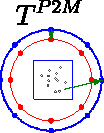
\includegraphics[height=2.1cm]{ch_1/kifmm2.pdf}
    \end{center} 
    \vspace{2pt} 

    This is matched to $N_e$ `equivalent charges', $\mathsf{q}^e$, placed evenly on a the (red) equivalent surface at $\{ x_i \}_i^{N_e}$. These surfaces are taken to be circles in $\mathbb{R}^2$ and cubes in $\mathbb{R}^3$. They perform a Tikhonov-regularised least squares fit to calculate  $\mathsf{q}^e$, which plays the role of the \textit{multipole expansion}.
    
    \begin{flalign*}
        \mathsf{q}^e = (\alpha I + \mathsf{K}^* \mathsf{K})^{-1}\mathsf{K}\mathsf{q}^{\text{node}}
    \end{flalign*}

    where $\mathsf{q}^{\text{node}}$ are the charges in the leaf node. Using a similar framework, involving equivalent and check surfaces, the $T^{M2M}$, $T^{M2L}$, $T^{L2L}$ and $T^{L2P}$ operators are also calculated with Tikhonov-regularised least squares fitting, and are sketched below.

    \vspace{2pt} 
    \begin{center}
        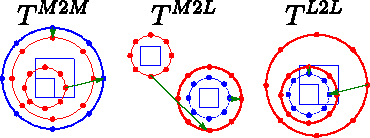
\includegraphics[height=2.1cm]{ch_1/kifmm.pdf}
    \end{center} 
    \vspace{2pt} 

    The KIFMM is designed for non-oscillatory kernels, such as the Laplace kernel of our didactic example, though in practice works well with low-frequency oscillatory problems, with extensions to high frequency problems \cite{engquist2007fast}.
    
    The least-squares fit can be pre-computed for each given geometry, and re-used. Additionally, as the KIFMM decomposes into a series of matrix vector products, it is well suited to software implementations.
    \end{tcolorbox} 
        
    \columnbreak
    \begin{tcolorbox}[width=1\linewidth, halign=left, colframe=black, colback=gray!10, boxsep=2mm, arc=0mm, left=1pt,right=1pt,top=0pt,bottom=0pt]
    \textbf{Black-Box FMM (bbFMM)}
    
    \setlength{\belowdisplayskip}{0pt} \setlength{\belowdisplayshortskip}{0pt}
    
    \setlength{\abovedisplayskip}{0pt} \setlength{\abovedisplayshortskip}{0pt}


    An $n$ point interpolation scheme for the kernel is constructed sequentially over each variable, 

    \begin{flalign*}
        &K(x, y) \approx \sum_{l=1}^n K(x_l, y)w_l(x) \\
        &K(x, y) \approx \sum_{l=1}^n\sum_{m=1}^nK(x_l, x_y)w_l(x)w_m(x)
    \end{flalign*}

    with coefficients $w_l(x)$ and $w_m(x)$. The bbFMM uses first kind Chebyshev polynomials, $T_n$ to interpolate the kernel, defined as,

    \begin{flalign*}
        T_n(x) = \cos(n \theta), \> \> \text{where } x = \cos(\theta)
    \end{flalign*}

    over the closed interval $x \in [-1, 1]$. The roots, $\{ \bar{x}_m \}$ , known as Chebyshev nodes are defined as,

    \begin{flalign*}
        \bar{x}_m = \cos(\theta_m) = \cos(\frac{(2m-1\pi)}{2n}) \\
    \end{flalign*}
    
    This is a well known, stable, uniformly convergent, interpolation scheme, that doesn't suffer from Runge's phenomenon \cite{fong2009black}. An $n$ point Chebyshev approximation to a given function, $g(x)$ with $p_{n-1(x)}$, can be written as,

    \begin{flalign*}
        &p_{n-1}(x) = \sum_{k=1}^{n-1}c_k T_k(x) \\
        \text{where, } &c_k = \begin{cases}
            \frac{2}{n} \sum_{l=1}^ng(\bar{x}_l)T_k(\bar{x}_l), \text{ if } k > 0\\
            \frac{1}{n} \sum_{l=1}^ng(\bar{x}_l), \text{ if } k = 0
        \end{cases}
    \end{flalign*}

    we recognise,

    \begin{flalign*}
        &p_{n-1}(x) = \sum_{l=1}^ng(\bar{x}_l)S_n(\bar{x}_l, x) \\
        \text{with, } &S_n(x, y) = \frac{1}{n} + \frac{2}{n}\sum_{k=1}^{n-1}T_k(x)T_k(y)
    \end{flalign*}

    When applied to our generic interpolation for the kernel,

    \begin{flalign*}
        K(x, y) &\approx\\
        &\sum_{l=1}^n\sum_{m=1}^n K(\bar{x}_l, \bar{y}_m) S_n(\bar{x}_l, x) S_n(\bar{y_m}, y)
    \end{flalign*}

    which can be substituted into (\ref{eq:ch_2:two_box_calc}), recovering linear complexity as long as the number of Chebyshev nodes is small, $n \ll N$.

    \end{tcolorbox}

\end{multicols}
\noindent\begin{minipage}{\textwidth}
    \captionof{figure}{The formulations of the kernel-independent FMM methods, the KIFMM \cite{Ying:2004:JCP} and the bbFMM \cite{fong2009black}.}
    \label{box:ch_2:kifmm_vs_bbfmm} 
\end{minipage}
